\section{Patterns of Enterprise Application Architecture (PoEAA)}
Martin Fowler created a good overview of \href{https://www.martinfowler.com/eaaCatalog/index.html}{PoEAA}. The book is from 2003, logical layers and most base patterns are still valid until today. 

\subsection{Presentation Layer Pattern}
The template view pattern is used in distributed presentation and the Template View Pattern is one example of a Presentation layer Pattern. The known uses are in: JavaScript (Handlebars), ASP.NET, JSPs.

\begin{figure}[H]
  \center
  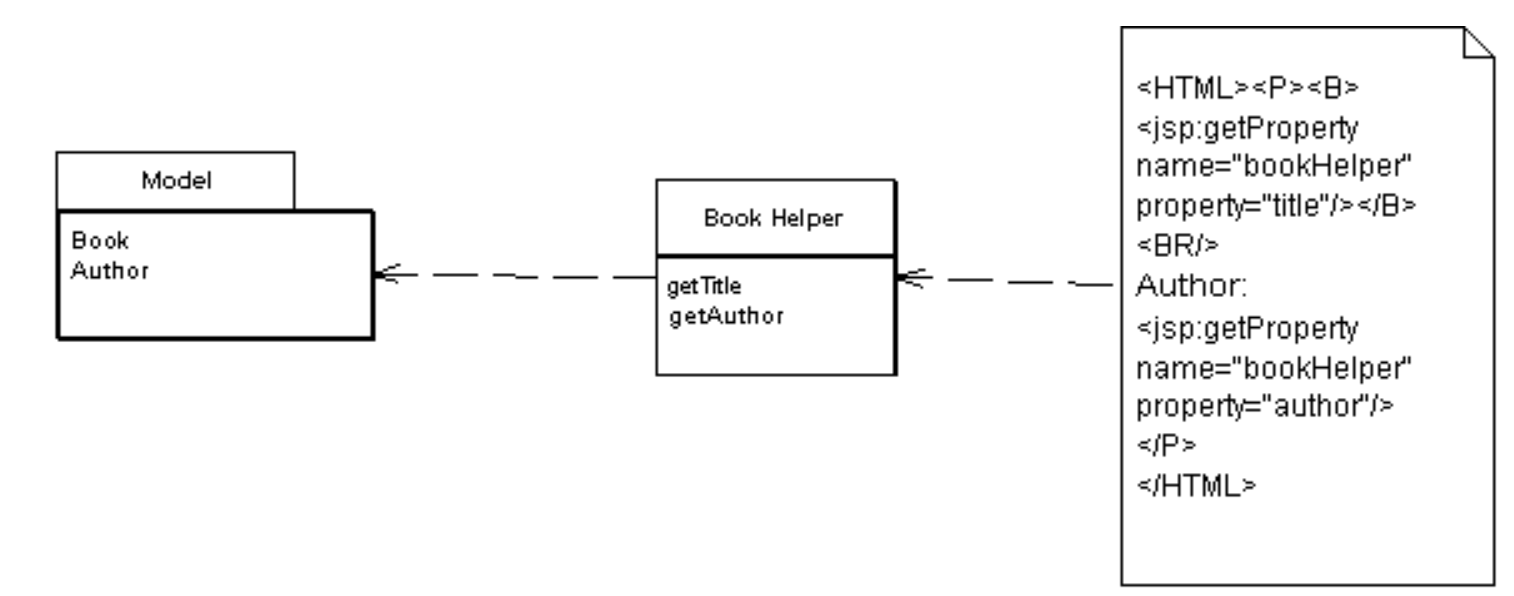
\includegraphics[width=0.75\textwidth]{templateviewpattern}
  \caption{Template View Pattern}
\end{figure}

\subsection{Domain Model Pattern}
The domain model is an object of the domain that incorporates both behaviour and data. At its worst business logic can be very complex. Rules and logic describe many different cases and slants of behaviour, and it's this complexity that objects were designed to work with. A Domain Model creates a web of interconnected objects, where each object represents some meaningful individual, whether as large as a corporation or as small as a single line on an order form.

\begin{figure}[H]
  \center
  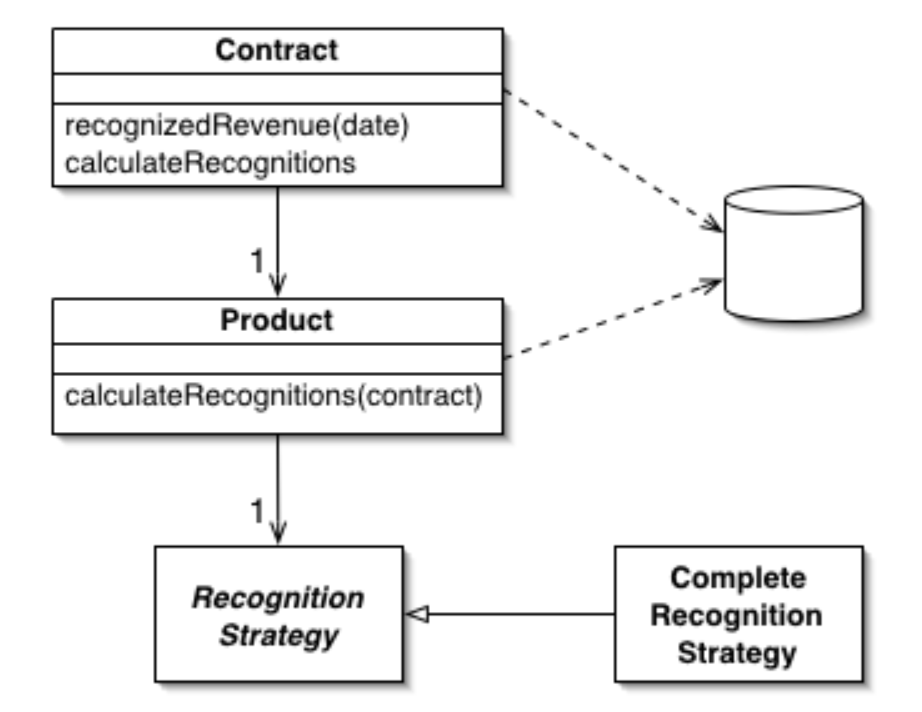
\includegraphics[width=0.5\textwidth]{domainmodelpattern}
  \caption{Domain Model Pattern}
\end{figure}

\section{Domain Driven Design}
DDD is a major software design concept introduced by the programmer Eric Evans in 2004, focusing on modelling software to match a domain according to input from that domain's expert. Properly applied it can lead to software abstractions called domain models. These models encapsulate complex business logic, closing the gap between business reality and code. It does this by analysing the problem first in a top-down approach.

The main advantages of using Domain-Driven Design is: it improves our craft, it provides flexibility, it prefers domains over interfaces, it reduces communication gaps between teams through ubiquitous language. On the other hand the disadvantages are: it requires a professional with strong domain expertise, it encourages the team to follow iterative practices.

\begin{figure}[H]
  \center
  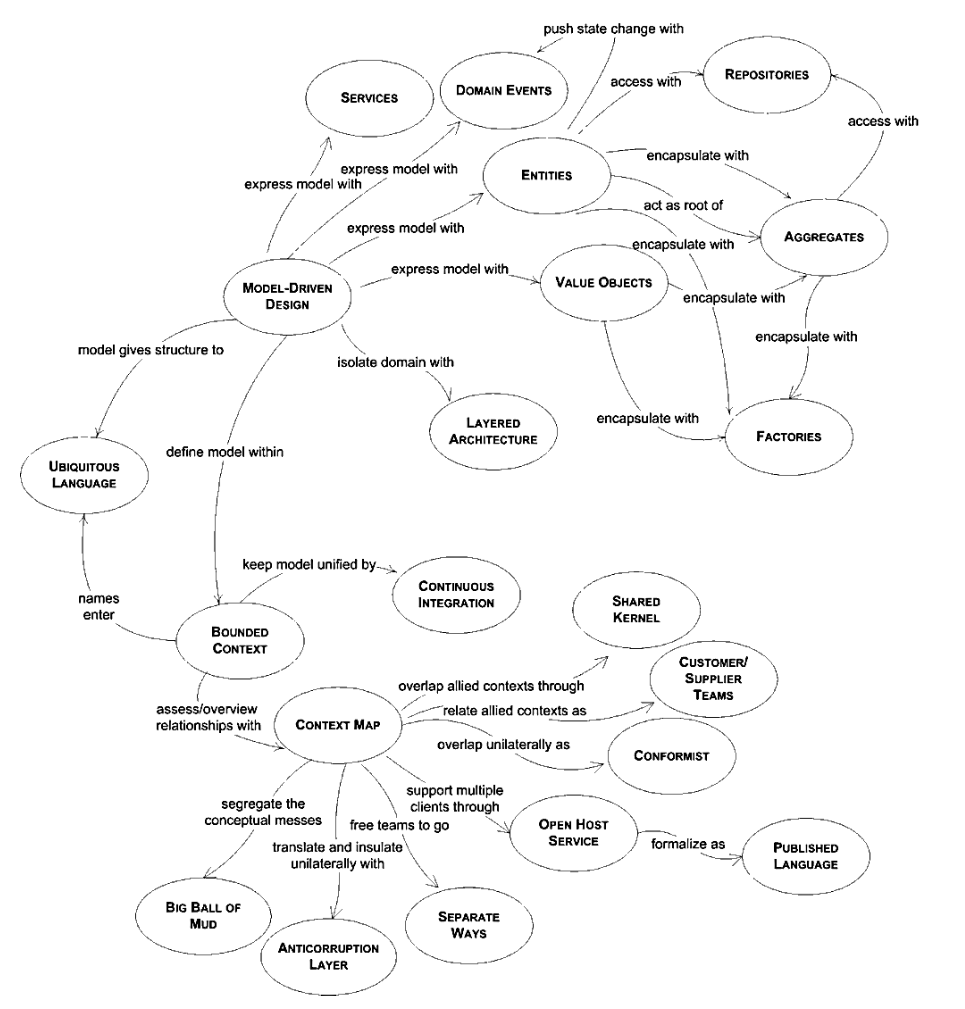
\includegraphics[width=0.8\textwidth]{patternlanguage}
  \caption{Pattern Language Overview}
\end{figure}


\paragraph{Tactical and Strategic Design} \hfill \\
Domain-driven design knows two types of design tools: Strategic design tools and Tactical design tools. The developers usually use tactical design tools and should have a good understanding of strategic design tools in order to architect good software.

\pagebreak

\subsection{Strategic Design}
Strategic Design helps the developer to solve all problems regarding software modelling. It has similarities to Object-oriented design. In strategic design the architect is also forced to think in terms of a context.

\begin{description}
	\item [Domain] a sphere of knowledge or activity and refers to the business. 
	\item [Model] a system of abstractions representing selected aspects of a domain.
	\item [Ubiquitous Language] Is a common language used by all team members to describe activities of the team around the domain model. It is used to to talk with domain experts and team members and describe classes, methods etc.
	\item [Bounded Context] Refers to a boundary condition for a context. It descends a boundary and acts as a threshold within which, a particular domain model is defined and applicable. \textit{Heuristic:} Implement one (micro-)service per Bounded Context
\end{description}

\subsubsection{Bounded Context vs. Subdomain}
Bounded Contexts implement parts of one or multiple subdomains. 

\begin{description}
	\item [Subdomain] is in the problem space and the result of Object-oriented analysis (OOA)
	\item [Bounded Context] is in the solution space and the result of Object-oriented design (OOD)
\end{description}

\subsubsection{Bounded Context Map}
The Context Map as in Figure \ref{fig:contextmap} defines how Bounded Contexts do integrate. Additionally the information flow between the context is modelled.  To create Such Context Maps the \href{https://contextmapper.org/}{Context Mapper} can be used.

\begin{description}
	\item [Shared Kernel] Two bounded contexts use a common kernel of code (for example a library) as a common lingua-franca, but otherwise do their other stuff in their own specific way. This is a symmetric relationship.
	\item [Open Host Service (OHS)] A Bounded Context specifies a protocol by which any other bounded context can use its services (e.g. a RESTful HTTP service or a SOAP Web service). This protocol may expose a Published Language.
	\item [Published Language (PL)] The interacting bounded contexts agree on a common a language (for example a bunch of XML or JSON schemas over an enterprise service bus) by which they can interact with each other. 
	\item [Conformist (CF)] One BC uses the services of another but is not a stakeholder to that other BC. As such it uses "as-is" (conforms to) the protocols or APIs provided by that bounded context (which may be an OHS).
	\item [Anti-Corruption Layer (ACL)] One bounded context uses the services of another and is not a stakeholder, but aims to minimize impact from changes in the bounded context it depends on by introducing a set of adapters – an anti-corruption layer.
	\item [Customer/Supplier (CS)]  One bounded context uses the services of another and is a stakeholder (customer) of that other bounded context. As such it can influence the services provided by that bounded context. The supplier may expose a PL.
\end{description} 

\begin{figure}[H]
  \center
  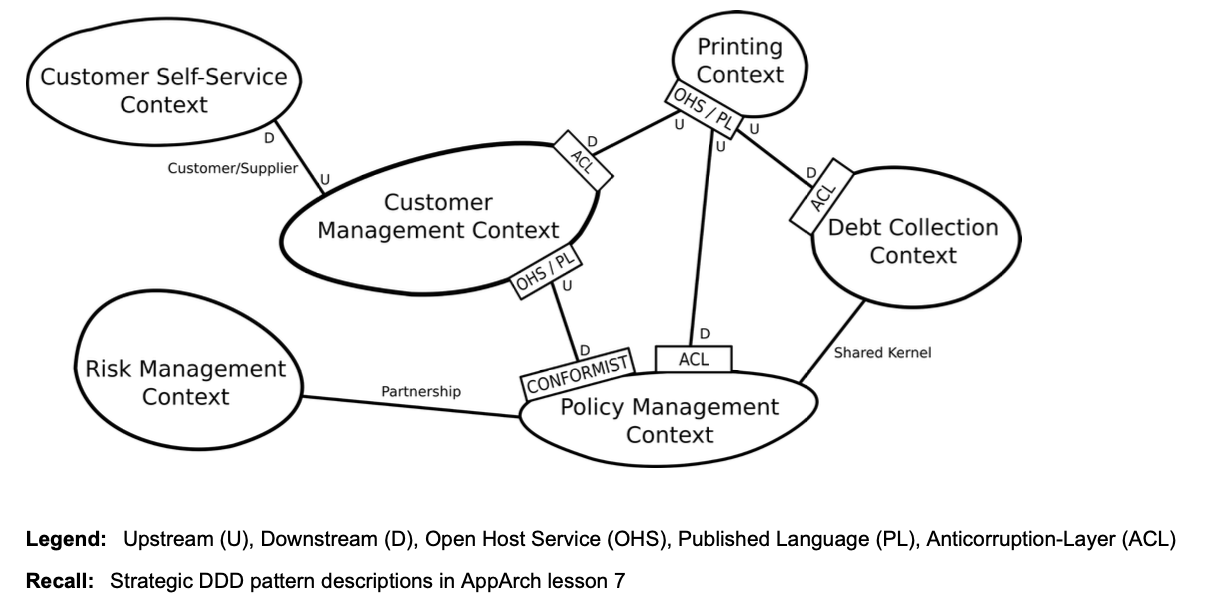
\includegraphics[width=0.65\textwidth]{contextmap}
  \caption{Bounded Context Example}
  \label{fig:contextmap}
\end{figure}

\pagebreak

\subsection{Tactical Design}
In contrast to the strategic design, tactical design talks about implementation details. It takes care of component inside a bounded context. Known artefact's such as services, entities, and factories are defined in this step. This process occurs during the product development phase.

Parts of the domain model created in the Tactical design phase:
\begin{description}
	\item [Entity] An Entity is a class which has some properties. Each instance of the class has a global identity and keeps the identity throughout the lifespan.
	\item [Value Object] Are \textit{immutable} and light-weight objects without an identity. 
	\item [Service] A service is a stateless class that fits somewhere else other than an entity or value object. A service is a functionality that exists somewhere between entities and values objects but it is neither related to an entity nor values objects.
	\item [Aggregate] An Aggregate is a collection of entities and values which come under a single transaction boundary.
	\item [Repository] A Repository helps in persisting aggregates.
	\item [Factory] A Factory does create aggregates in order for them to be used in the application.
\end{description}

\begin{figure}[H]
  \center
  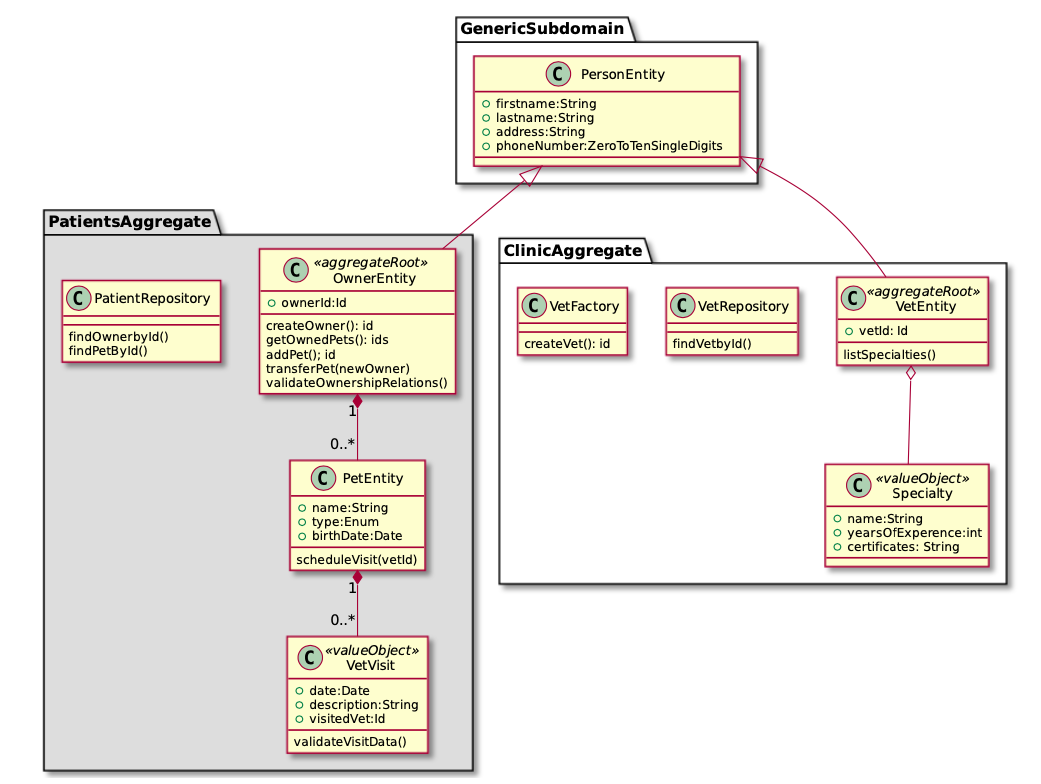
\includegraphics[width=0.9\textwidth]{tacticddd}
  \caption{Tactic DDD Model}
\end{figure}

\section{Component Responsibility Collaborators Cards (CRCs)}
CRC cards are used to propose architectural elements, describe their responsibilities and show how they are combined together to from an architecture. This breaks down the functionality of an application to the basic entities (class), what the have to do (responsibly) and with which other entities hey communicate (collaborator).

\begin{figure}[H]
  \center
  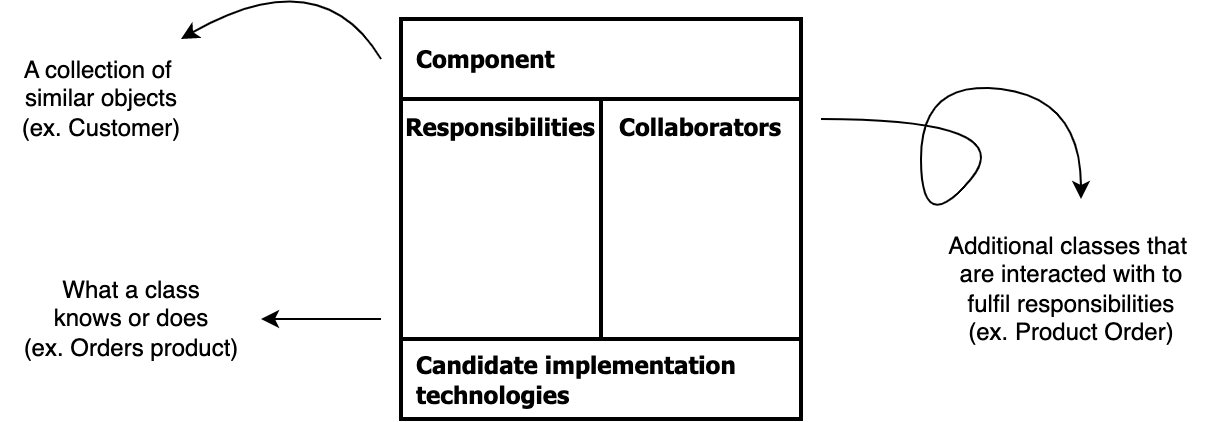
\includegraphics[width=0.85\textwidth]{crc}
  \caption{CRC Card Tempalte}
\end{figure}

The following CRC card in Figure \ref{fig:crcexample} shows a filled out example from the \href{https://spring-petclinic.github.io/}{Spring PetClinic}.

\begin{figure}[H]
  \center
  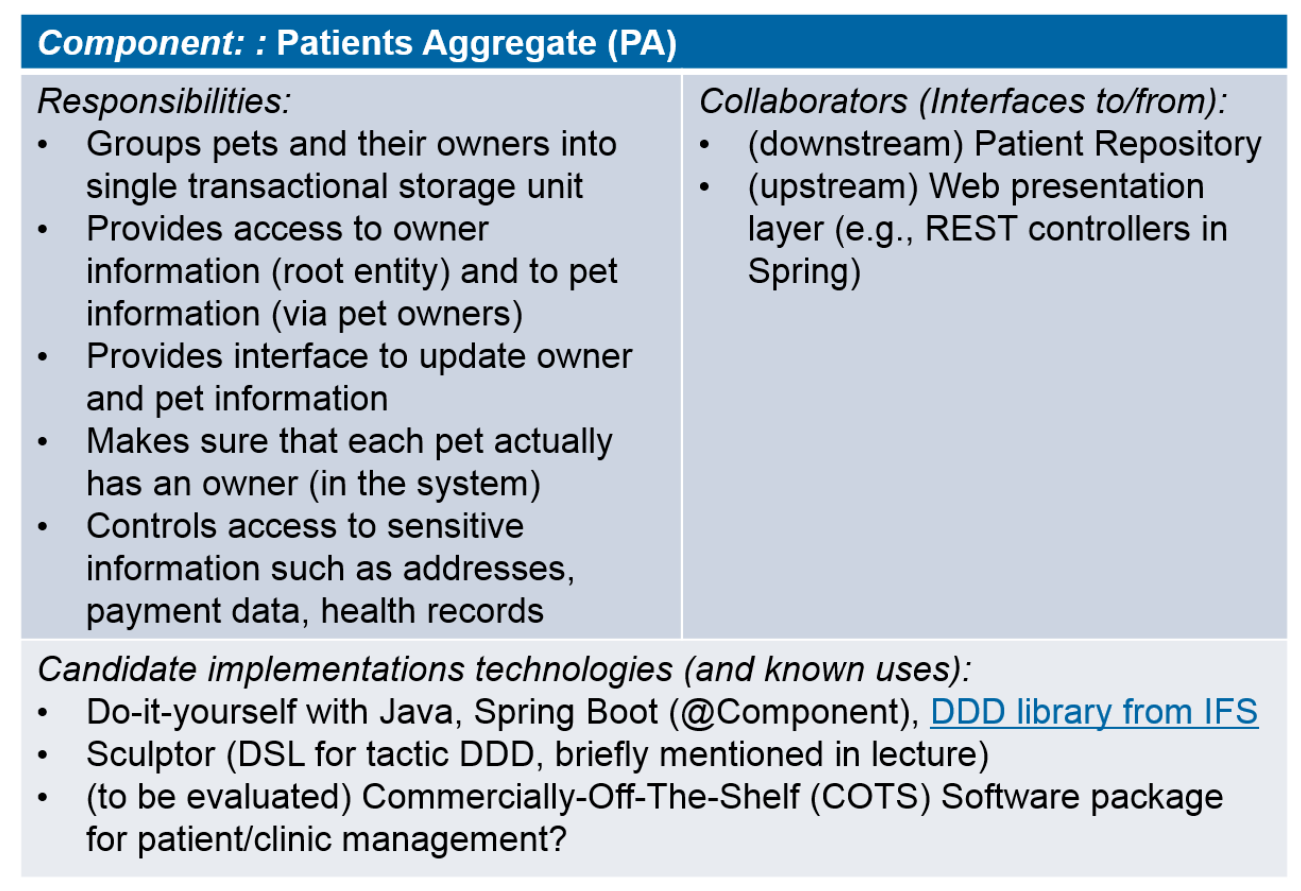
\includegraphics[width=0.75\textwidth]{crcexample}
  \caption{CRC Example for PetClinic}
  \label{fig:crcexample}
\end{figure}

